\documentclass[12pt,a4paper]{article}
\usepackage[a4paper,left=3cm,right=3cm,top=2.5cm,bottom=2.5cm]{geometry}

\usepackage{fontspec}
\setmainfont{Times New Roman}
\usepackage{graphicx}
\usepackage{xcolor}
\usepackage{hyperref}
\newcommand{\noindentfix}{\vspace{10pt}\noindent}
\newcommand{\chapterheader}[1]{{\noindent\fontsize{18}{14}\textbf{#1}\vspace{2pt}}}
\newcommand{\subchapterheader}[1]{{\noindent\fontsize{16}{14}\textbf{#1}\vspace{2pt}}}
\newcommand{\HighlightedTextLightgray}[1]{\texttt{\colorbox{gray!30}{#1}}}

\usepackage{listings}

\usepackage{polyglossia}
\setdefaultlanguage{slovak}
\setotherlanguage{english}


\renewcommand{\lstlistingname}{Zdrojový kód} % Listing -> Algorithm

\usepackage{xcolor}
\definecolor{codegreen}{rgb}{0,0.6,0}
\definecolor{codegray}{rgb}{0.5,0.5,0.5}
\definecolor{codepurple}{rgb}{0.58,0,0.82}
\definecolor{codeorange}{rgb}{1,0.5,0}
\definecolor{codemagenta}{rgb}{1,0,0.5}
\definecolor{codedarkblue}{rgb}{0,0,0.5}
\definecolor{backcolour}{rgb}{0.95,0.95,0.92}

% https://tex.stackexchange.com/questions/110722/trying-to-include-r-code-with-listings-package
\definecolor{dkgreen}{rgb}{0,0.6,0}
\definecolor{gray}{rgb}{0.5,0.5,0.5}
\definecolor{mauve}{rgb}{0.58,0,0.82}
\lstset{ %
  language=java,                     % the language of the code
  basicstyle=\footnotesize,       % the size of the fonts that are used for the code
  numbers=left,                   % where to put the line-numbers
  numberstyle=\tiny\color{gray},  % the style that is used for the line-numbers
  stepnumber=1,                   % the step between two line-numbers. If it's 1, each line
                                  % will be numbered
  numbersep=8pt,                  % how far the line-numbers are from the code
  backgroundcolor=\color{white},  % choose the background color. You must add \usepackage{color}
  showspaces=false,               % show spaces adding particular underscores
  showstringspaces=false,         % underline spaces within strings
  showtabs=false,                 % show tabs within strings adding particular underscores
  frame=single,                   % adds a frame around the code
  rulecolor=\color{black},        % if not set, the frame-color may be changed on line-breaks within not-black text (e.g. commens (green here))
  tabsize=4,                      % sets default tabsize to 2 spaces
  captionpos=b,                   % sets the caption-position to bottom
  breaklines=true,                % sets automatic line breaking
  breakatwhitespace=false,        % sets if automatic breaks should only happen at whitespace
  title=\lstname,                 % show the filename of files included with \lstinputlisting;
                                  % also try caption instead of title
  keywordstyle=\color{blue},      % keyword style
  commentstyle=\color{dkgreen},   % comment style
  stringstyle=\color{mauve},      % string literal style
  escapeinside={\%*}{*)},         % if you want to add a comment within your code
  morekeywords={*,...}            % if you want to add more keywords to the set
} 

\begin{document}

    \begin{flushleft}
        \begin{center}
            \MakeUppercase[]{
                \vspace{0.5cm}{
                    \noindent\expandafter\footnotesize{Fakulta prírodných vied Univerzity Mateja Bela v Banskej Bystrici}
                }
            }
            \thispagestyle{empty}
            \MakeUppercase[]{
                \noindent
                \vfill
                \vspace{10pt}{
                    \noindent\expandafter\fontsize{30}{25}\textbf{Dokumentácia} \\
                }
                \vspace{30pt}
            }
            \MakeUppercase[]{
                \noindent
                \vspace{25pt}{
                    \noindent\expandafter\fontsize{14}{15}\textbf{Akceptor pre konkrétny regulárny výraz} \\
                }
            }
            {
                \vspace{50pt}    
                \noindent\\{15. novembra 2024}
            }
        \end{center}
        \thispagestyle{empty}
        \vfill
        \noindent
        \begin{tabular}{ll}
            Jakub Kubaliak              \\
            122nAIm, 1. ročník              \\
            Formálne jazyky a automaty    \\
        \end{tabular}
    \end{flushleft}
    \newpage

    \chapterheader{Spustenie aplikácie}

    \noindentfix Odkaz na Github repozitár: \textcolor{cyan!80}{\href{https://github.com/Voltrifrodec/formalne-jazyky-a-automaty}{https://github.com/Voltrifrodec/formalne-jazyky-a-automaty}}
    
    \noindentfix Vytvorenie .jar súboru a spustenie aplikácie (môže vyžadovať nainštalovaný \HighlightedTextLightgray{mvn}; spúšťame v priečinku \HighlightedTextLightgray{/aplikacia}):

    \noindentfix \fcolorbox{black}{gray!30}{
        \parbox{\linewidth}{
            \texttt{mvn clean package}\linebreak\texttt{java -jar ./target/zadanie1-1.0.jar}
        }
    }

    \noindentfix Manuálne zadanie vstupu:

    \noindentfix \fcolorbox{black}{gray!30}{
        \parbox{\linewidth}{
            \texttt{java -jar ./target/zadanie1-1.0.jar}
        }
    }

    \noindentfix Zadanie vstupu zo súboru:

    \noindentfix \fcolorbox{black}{gray!30}{
        \parbox{\linewidth}{
            \texttt{java -jar ./target/zadanie1-1.0.jar test-retazcov.txt}
        }
    }

    \noindentfix Spustenie testov:

    \noindentfix \fcolorbox{black}{gray!30}{
        \parbox{\linewidth}{
            \texttt{mvn test}
        }
    }
    \pagebreak

    \chapterheader{Rozbor riešenia}

    \noindentfix Môj regulárny výraz bol výraz \HighlightedTextLightgray{[a]b\{a|b\}}:
    \begin{figure}[h]
        \centering
        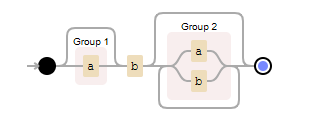
\includegraphics{./assets/stavovy-diagram-pre-regularny-vyraz.png}
        \caption{Stavový diagram pre regulárny výraz \HighlightedTextLightgray{(a)?b(a|b)*}.}
        \label{fig:stavovy-diagram}
    \end{figure}

    \noindentfix Teda, na prvej pozícii sa vyskytuje 0 alebo 1 znakov \HighlightedTextLightgray{a}, nasleduje jeden znak \HighlightedTextLightgray{b} a potom sa vyskytuje 0 alebo viac znakov \HighlightedTextLightgray{a} alebo \HighlightedTextLightgray{b}.

    \noindentfix Akceptovanými reťazcami môže byť napríklad:
    \begin{itemize}
        \setlength{\parskip}{0pt}
        \setlength{\itemsep}{0pt}
        \item \HighlightedTextLightgray{ab}
        \item \HighlightedTextLightgray{abba}
        \item \HighlightedTextLightgray{b}
        \item \HighlightedTextLightgray{bba}
    \end{itemize}

    \noindentfix Naopak neakceptovanými reťazcami môžu byť:
    \begin{itemize}
        \setlength{\parskip}{0pt}
        \setlength{\itemsep}{0pt}
        \item \HighlightedTextLightgray{a}
        \item \HighlightedTextLightgray{aabb}
        \item \HighlightedTextLightgray{aa}
        \item \HighlightedTextLightgray{aab}
    \end{itemize}

    \noindentfix Pri riešení zadania som sa rozhodol pre programovací jazyk Java a využiť nástroj Maven pre testovanie výrazov.

    \noindentfix Ako prvú vec, ktorú som urobil, bolo vytvorenie nového Maven projektu. Najprv som vytvoril konfiguračný súbor \HighlightedTextLightgray{pom.xml}, do ktorého som nastavil základné parametre pre projekt (názov, verziu Javy a pod.) a následne inicializoval vytvorený projekt príkazom \HighlightedTextLightgray{mvn clean install}. Potom som pracoval na vytvorení algoritmu, príslušných unit testov a následne pridanie podpory pre vstup z konzoly a textového súboru.

    \pagebreak
    \subchapterheader{Algoritmus}

    \noindentfix Zo zadania som vyčítal, že nemôžem použiť knižnice pre regulárne výrazy. Pre riešenie je možné využiť buď jeden cyklus \HighlightedTextLightgray{while}, počas ktorého budem odoberať zo vstupného reťazca znaky podľa stavu, alebo využiť rekurzívne funkcie a tým elimininovať potrebu cyklu. V riešení som sa rozhodol pre využitie cyklu \HighlightedTextLightgray{while}.

    \noindentfix Reťazec som overoval po častiach. Najprv som overil či nie je reťazec prázdny. Následne som overil prvý stav $q_0$ (reťazec obsahuje 0 alebo 1 počet znakov \HighlightedTextLightgray{a}). Po overení stavu $q_0$ som začal overovať druhý stav, $q_1$ (musí obsahovať znak \HighlightedTextLightgray{b}). Ako posledné som pomocou cyklu overoval posledný stav $q_2$ (reťazec obsahuje 0 alebo 1 počet znakov \HighlightedTextLightgray{a} alebo \HighlightedTextLightgray{b}).

    \noindentfix Nasledujúci zdrojový kód obsahuje hlavnú časť programu -- metódu obsahujúcu algoritmus pre akceptor. 

    \begin{center}
        \lstinputlisting[basicstyle=\scriptsize, language=java, caption={Ukážka vytvorenej metódy \HighlightedTextLightgray{compareToRegex}.}, label={lst:compare-to-regex}]{./assets/compare-to-regex.java}
    \end{center}

\end{document}